\section{运行背景与信任基础}
\subsection{异构任务体系}\label{sec:coalition}

UAV 提供快速重定位、视距无线电中继和光电感知。USV 携带更多能源和较大型天线，并连接声学与无线电网络。UUV 在水下目标附近作业，但大规模传输通常依赖低速声学链路，或延迟至上浮后进行。通信综述描述了由此产生的距离、带宽、时延、能耗与对准要求之间的权衡\citep{nomikos2023survey,ali2020recent,saeed2019underwater,jahanbakht2021internet}。拓扑、时钟质量和可达性可能在一次任务内发生变化。

考虑一个民用沿岸响应联盟，由主管机构 A、科研运营方 B、通信提供方 C 和签约数据提供方 D 组成。B 运行 UUV 和 UAV；C 提供 USV 中继；A 批准任务权限；D 提供独立数据和审计服务。各组织保留自身的管理身份。本地运营方可以认证设备，却可能无权改变联盟成员资格、证据策略或撤销历史。第~\ref{sec:trace} 节和第~\ref{sec:pattern} 节使用该联盟案例，明确哪些变更需要共同批准。

USV 可以同时承担声学流量中继、数据缓存、授时和融合计算。该共享依赖点发生故障，会影响若干表面上相互独立的数据产品。端到端源签名可在经过不可信中继时保留来源完整性，但选择性扣留，以及共同的时钟或转换错误仍需考虑。图~\ref{fig:architecture} 区分了受限证据路径与岸端共享状态服务。

原始图像、声呐数据、详细遥测和证明证据以加密形式保留在链下。共享记录包含承诺、成员资格、策略/模型版本、撤销信息和审计判断。容迟转发可使用 Bundle Protocol 第 7 版，以及 BPSec 的完整性与保密服务\citep{rfc9171,rfc9172}。存储转发机制使消息得以跨接触时段保存和传递；权限到期与证据年龄策略是独立的应用规则。

\subsection{任务信任与依赖决策}

\emph{任务信任}是根据可用证据和错误后果，在特定情境下决定是否为某个明确目的依赖某个对象。\emph{可信赖性}指支撑这一决定的属性：身份、测得的端点状态、链路可用性、溯源、时效性、观测质量，以及可问责的治理。同一幅图像可能适用于总体态势感知，却不适用于避碰。

对于对象 $o$、时间 $t$、情境 $c$ 和任务用途 $m$，评估与决策具有不同的接口：
\begin{equation}\begin{aligned}
T_o(t,c,m)&=\mathcal{A}(o,\mathcal{E}_{\leq t},c,m;\theta),\\
D_{r,o}(t,c,m)&=\pi_r\!\left(T_o(t,c,m),\mathcal{C}_t,m\right).
\end{aligned}\label{eq:trust}\end{equation}
其中，$\mathcal{E}_{\leq t}$ 包含截至决策时刻收到的证据，包括观测时间和谱系。评估函数 $\mathcal{A}$ 在假设 $\theta$ 下产生针对具体主张的结果及不确定性。依赖方 $r$ 在权限、截止时间、后果与资源约束 $\mathcal{C}_t$ 下，应用策略 $\pi_r$。结果可以是允许、限制、推迟或拒绝使用。主观意见、区间、有序状态和声誉值都可以实现该接口\citep{jsang2016subjective,mui2003computational,kamvar2003eigentrust}。若赋予概率解释，则需要明确的事件定义与校准证据。

\begin{figure}[!htbp]\centering
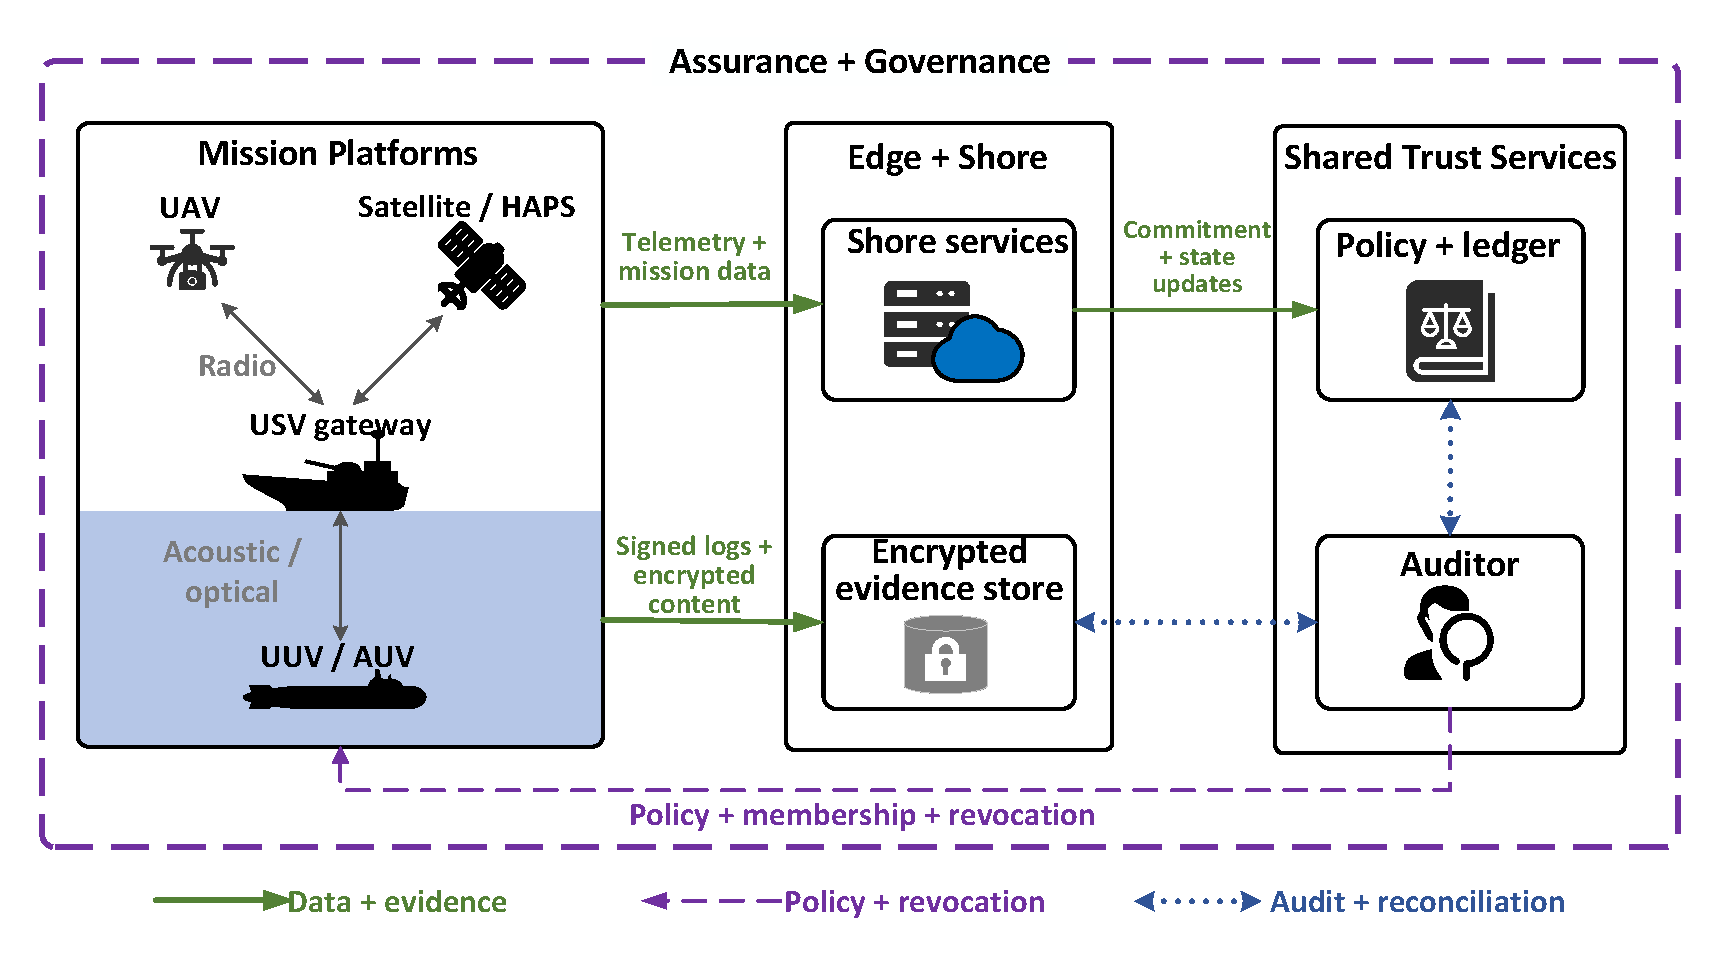
\includegraphics[width=\textwidth]{figures/figure-01-reference-architecture.pdf}
\caption{跨域参考架构。岸端组织部署对等节点与排序节点；USV 是转发/缓存依赖点。在网关分区期间，本地感知与安全控制在委托权限范围内继续运行。}\label{fig:architecture}
\end{figure}

\emph{可信数据环境}是产生、转换、共享和治理这些证据的社会技术环境。它包含主体、设备、路径、制品和问责流程。零信任提供以资源为中心的策略及执行机制\citep{rose2020zero}；OAL 则记录与任务依赖有关的附加观测、谱系、时间和后果主张。

\subsection{四类互补的保障主张}

观测有效性关注与物理世界的对应关系。承诺与溯源完整性关注受保护的字节，以及已记录的来源或转换过程。账本与治理一致性关注经过授权的共享状态转换。任务使用适合性关注特定的决策及其后果。图~\ref{fig:assurance-chain} 展示了这些不同问题及其支撑证据。

使用被盗密钥签名的伪造观测，可以通过签名验证。RATS 评估支撑限定范围的测量状态主张\citep{birkholz2023remote}，物理诊断与交叉佐证则支撑观测主张。依赖策略组合适用的结果，并明确规定要求未满足或状态未知时的响应。

\begin{figure}[!htbp]\centering
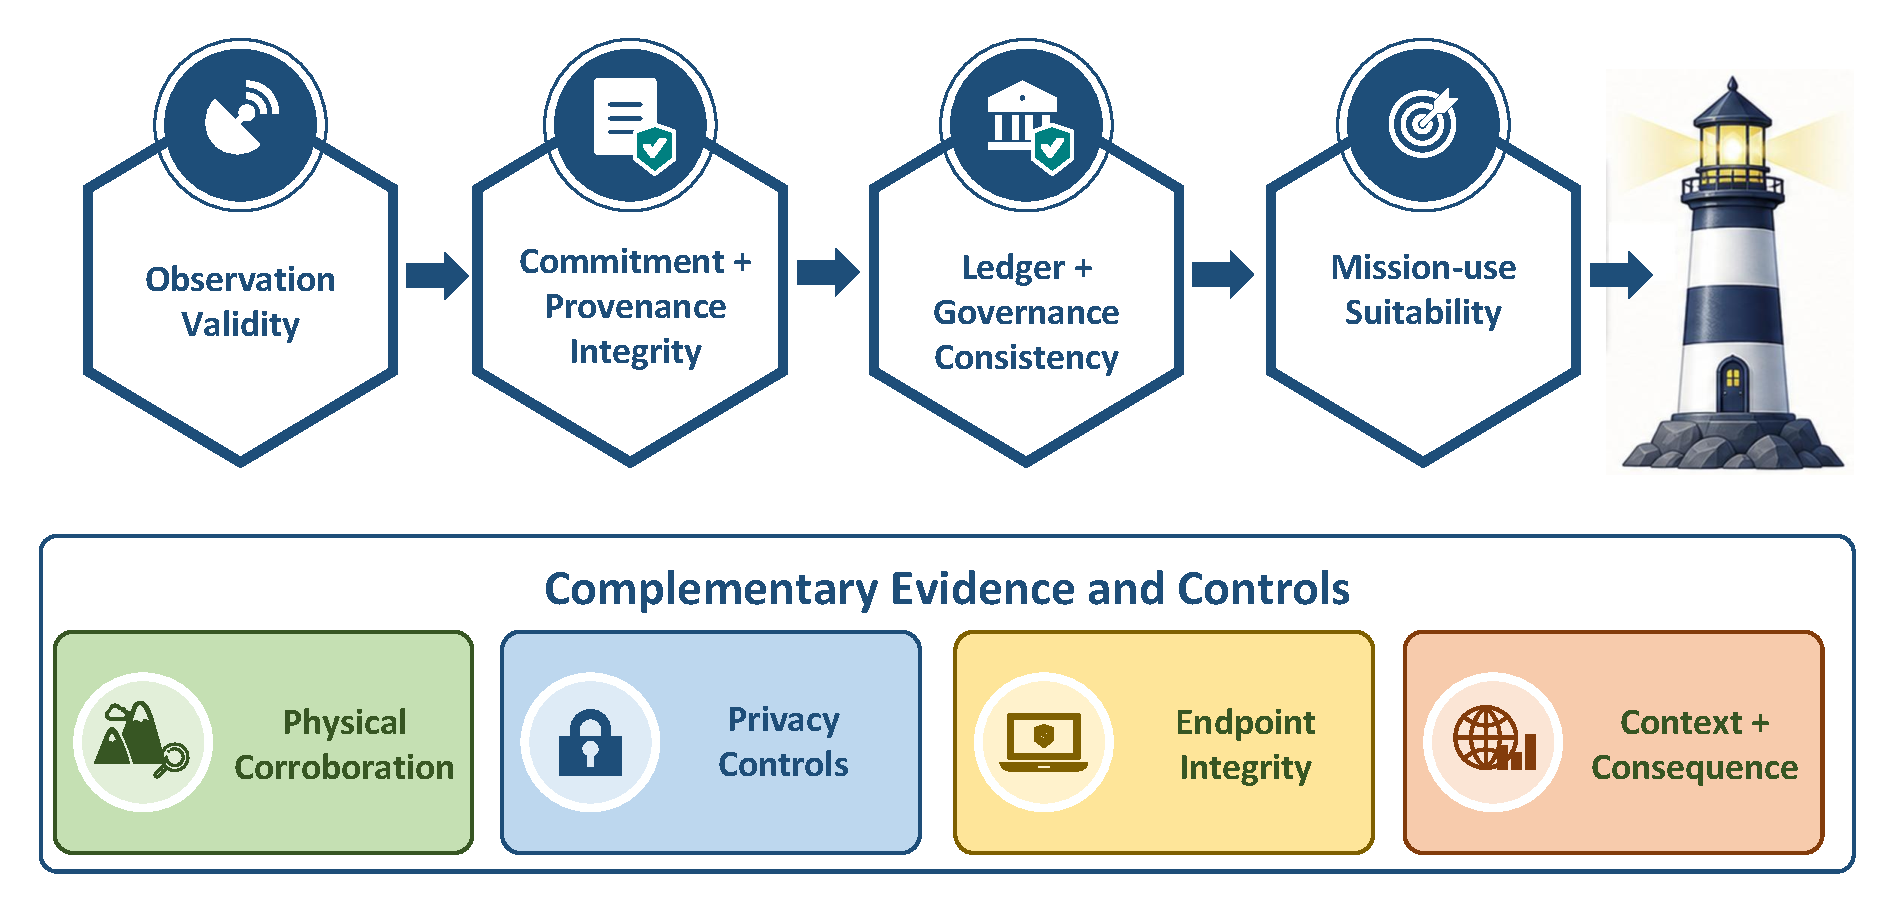
\includegraphics[width=\textwidth]{figures/figure-02-assurance-chain.pdf}
\caption{四类保障主张及其证据。图中的关系表示论证结构；实际实现可以按不同顺序执行检查。}\label{fig:assurance-chain}
\end{figure}
